\documentclass[10pt]{beamer}

% Metropolis Theme für den Beamer
% https://github.com/matze/mtheme
\usetheme{metropolis}
\usepackage{appendixnumberbeamer}
\setbeamertemplate{bibliography item}{[\theenumiv]}

% Eingabecodierung
\usepackage[utf8]{inputenc}

% Sprachraum
\usepackage[ngerman]{babel}

% Table einbinden
\usepackage{booktabs}
\usepackage[scale=2]{ccicons}

% Lücken/Buffer einbinden
\usepackage{xspace}
\newcommand{\themename}{\textbf{\textsc{metropolis}}\xspace}

% Bilder einbinden
\usepackage{graphicx}
\graphicspath{{images/}}

% Code einbinden
\usepackage{listings}

\title{Umgehung von Festplattenverschlüsselung mit Trusted Platform Module am Beispiel von BitLocker}
\subtitle{Professionelle Textsatzsysteme}
\date{\today}
\author{0xffd700}

\begin{document}
	
	\maketitle
	
	\begin{frame}{Inhaltsverzeichnis}
		\setbeamertemplate{section in toc}[sections numbered]
		\tableofcontents[hideallsubsections]
	\end{frame}

	
	\section{Festplattenverschlüsselung}
	
	\begin{frame}[fragile]{Festplattenverschlüsselung}
		
		\begin{quote}
			\centering
			Methode zum Schutz von Daten gegen physikalische Angriffe durch Verschlüsselung des gesamten Datenträgers oder einzelner Sektoren.
		\end{quote}
	\cite{SibingerChristophANDMullerTilo.2014}
		
	\end{frame}

	\begin{frame}[fragile]{Trusted Platform Module (TPM)}
		
		\begin{columns}[T,onlytextwidth]
			\column{0.5\textwidth}
			\begin{itemize}[<+- | alert@+>]
				\item Krypto-Prozessor zur Erweiterung von grundlegenden Sicherheitsfunktionen 
				\begin{itemize}
					\item Generiert, speichert und limitiert den Einsatz von kryptografischen Schlüsseln
					\item Authentifiziert Geräte
					\item Sicherstellung der Plattformintegrität
				\end{itemize}
			\end{itemize}
			
			\column{0.5\textwidth}
			\begin{figure}[h!]
				\centering
				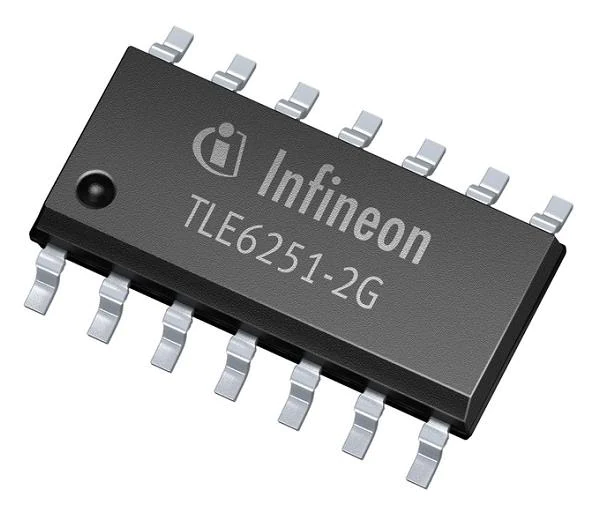
\includegraphics[width=0.8\linewidth]{TPM-Chip}
				\caption{TPM Chip \cite{.04102021}}
			\end{figure}
		\end{columns}
	\cite{TrustedComputingGroup.30072020}
	\end{frame}
	
	\begin{frame}[fragile]{BitLocker}
		
		\begin{columns}[T,onlytextwidth]
			\column{0.4\textwidth}
			\begin{itemize}[<+- | alert@+>]
				\item Sicherheitsfunktion von Microsoft 
				\item Plattformvalidierung durch Sealed Storage
				\item Entschlüsselung mit BitLocker:
				\begin{itemize}
					\item Volume Master Key (VMK)
					\item Storage Root Key (SRK)
					\item Full Volume Encryption Key (FVEK)
				\end{itemize}
			\end{itemize}
			
			\column{0.6\textwidth}
			\begin{figure}[h!]
				\centering
				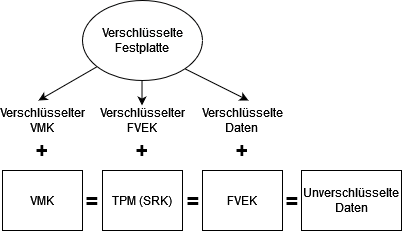
\includegraphics[width=0.8\linewidth]{BitLocker}
				\caption{BitLocker Entschlüsselung}
			\end{figure}
		\end{columns}
	\cite{Dansimp.13122021}
	\end{frame}
	
	
	\section{Umgehung von Festplattenverschlüsselung}
	
	\begin{frame}{Bekannte Angriffe}
		\begin{itemize}[<+- | alert@+>]
			\item Evil Maid Angriff
			\item Cold Boot Angriff
			\item Direkt Memory Access Angriff
			\item Hotplug Angriff
		\end{itemize}
	\cite{GuruprasadBidare.2017}
	\end{frame}
	
	\begin{frame}{Serial Peripheral Interface (SPI) Angriff}
		
		\begin{itemize}[<+- | alert@+>]
			\item FVEK wird beim Bootvorgang vom TPM zu Windows gesendet
			\item Unverschlüsselte Kommunikation zwischen TPM und CPU
			\item Auslesen der Daten über den SPI-Bus
		\end{itemize}
	\end{frame}
	
	
	\section{Praxisversuch}
	
	\begin{frame}{Versuchsaufbau}
		\begin{itemize}[<+- | alert@+>]
			\item Physikalischer Zugriff
			\item Windows 10 Professional
			\item Vollständige Verschlüsselung mit BitLocker
			\item TPM 2.0 mit Serial Peripheral Interface
		\end{itemize}
	\end{frame}
	
	\begin{frame}{Trusted Platform Module abhören}
			\begin{columns}[T,onlytextwidth]
			\column{0.5\textwidth}
			\begin{figure}[h!]
	\centering
	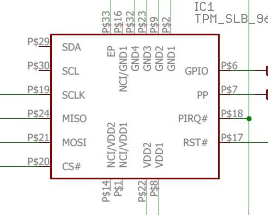
\includegraphics[width=0.9\linewidth]{infineon}
	\caption{Infineon TPM \cite{.15122021}}
\end{figure}
			\column{0.5\textwidth}
			\begin{figure}[h!]
				\centering
				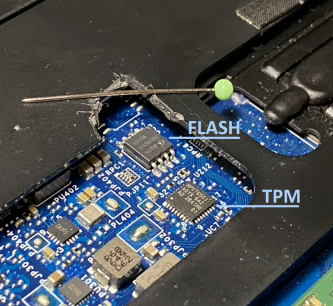
\includegraphics[width=0.8\linewidth]{flash-and-tpm}
				\caption{BIOS und TPM \cite{.16122020}}
			\end{figure}
		\end{columns}
	\end{frame}
	
	\begin{frame}{Serial Peripheral Interface}			
		\begin{columns}[T,onlytextwidth]
			\column{0.4\textwidth}
		\begin{itemize}[<+- | alert@+>]
	\item Synchroner und serieller Datenbus mit Master-Slave-Prinzip
	\item SPI-Bus:
	\begin{itemize}
		\item Master Out Slave In (MOSI)
		\item Master In Slave Out (MISO)
		\item Schiebetakt (CLK)
		\item Chip Select (CS)
	\end{itemize}
\end{itemize}
			\column{0.6\textwidth}
			\begin{figure}[h!]
				\centering
				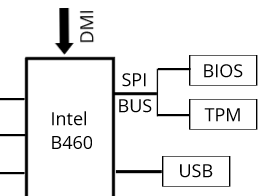
\includegraphics[width=0.8\linewidth]{SPI}
				\caption{SPI-Bus \cite{GIGABYTETECHNOLOGYCO.LTD.}}
			\end{figure}
		\end{columns}
	\cite[S. 335-349]{Wootton.2016}
	\end{frame}
	
	\begin{frame}{SPI-Bus abhören}
\begin{figure}[h!]
	\centering
	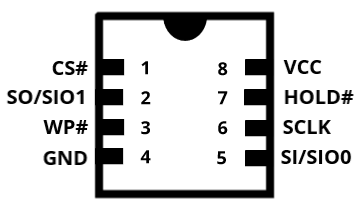
\includegraphics[width=0.8\linewidth]{BIOS}
	\caption{BIOS Blockdiagramm \cite{MacronixInternationalCo.LTD..2010}}
\end{figure}
	\end{frame}
	
	\begin{frame}{Logik Analyzer}
			\begin{figure}[h!]
			\centering
			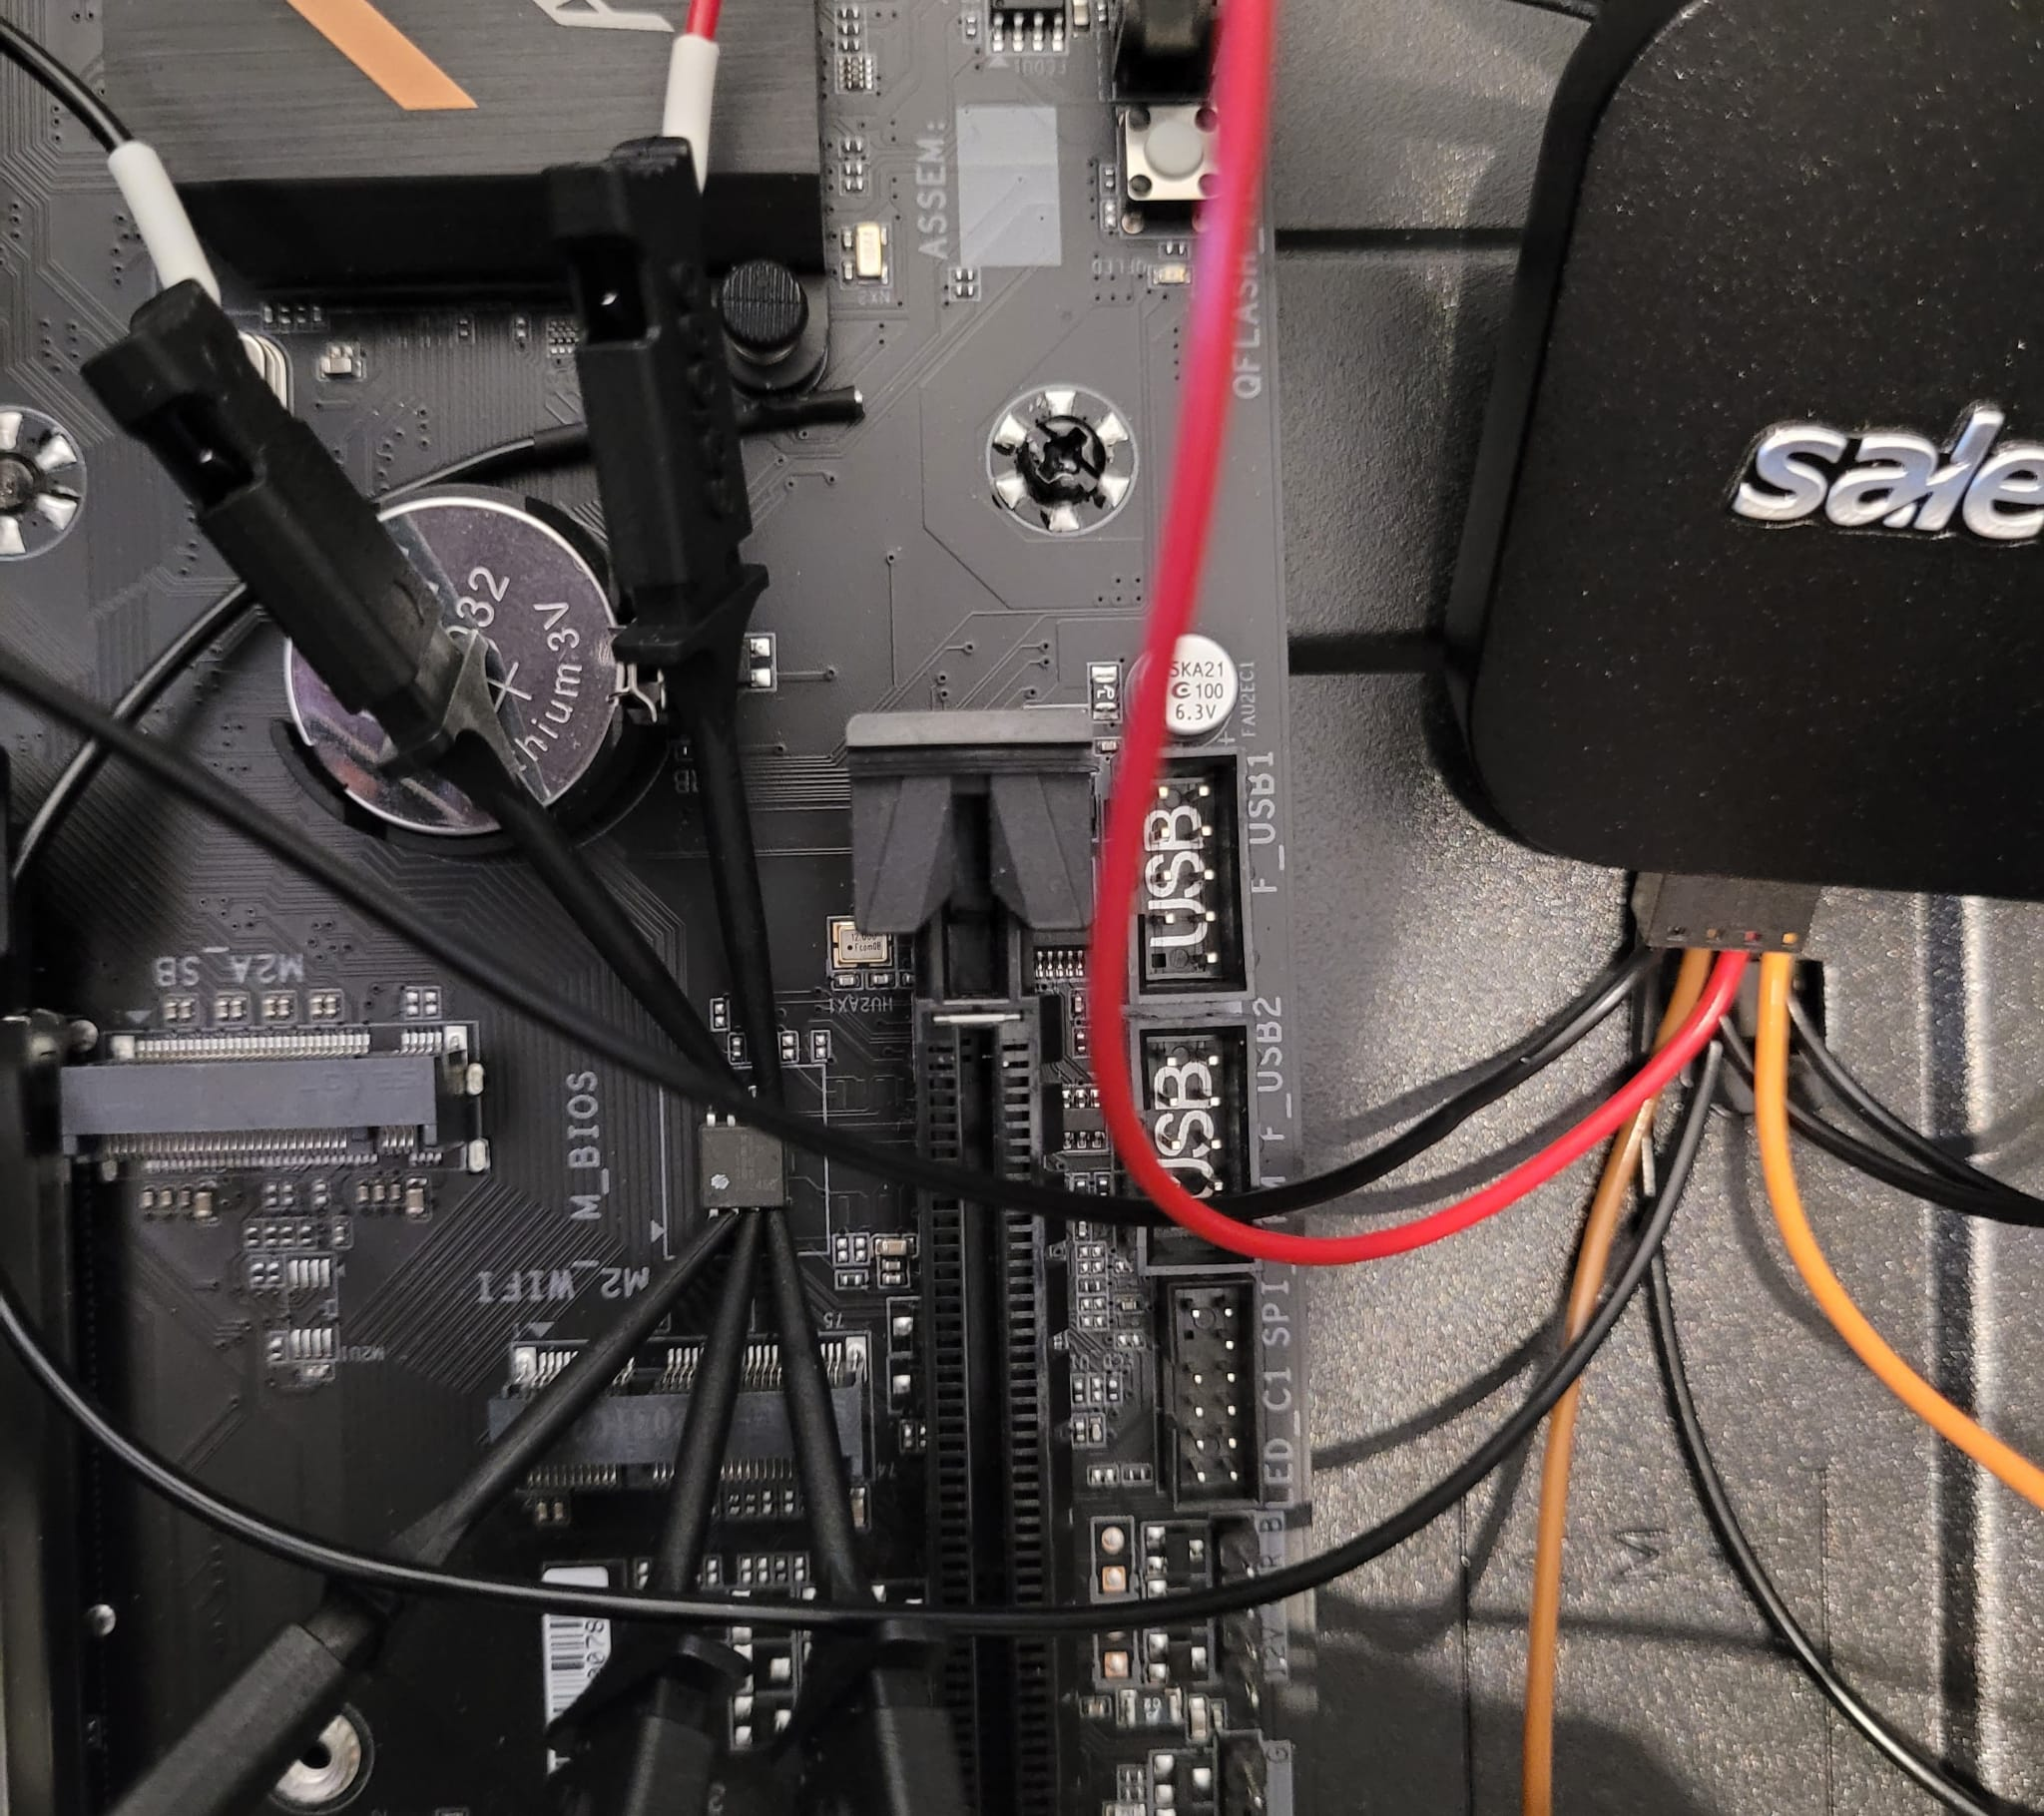
\includegraphics[width=0.6\linewidth]{Salea}
			\caption{Saleae Logik Analyzer}
		\end{figure}
	\end{frame}
	
	\begin{frame}{BitLocker Key Extractor}
		\begin{figure}[h!]
			\centering
			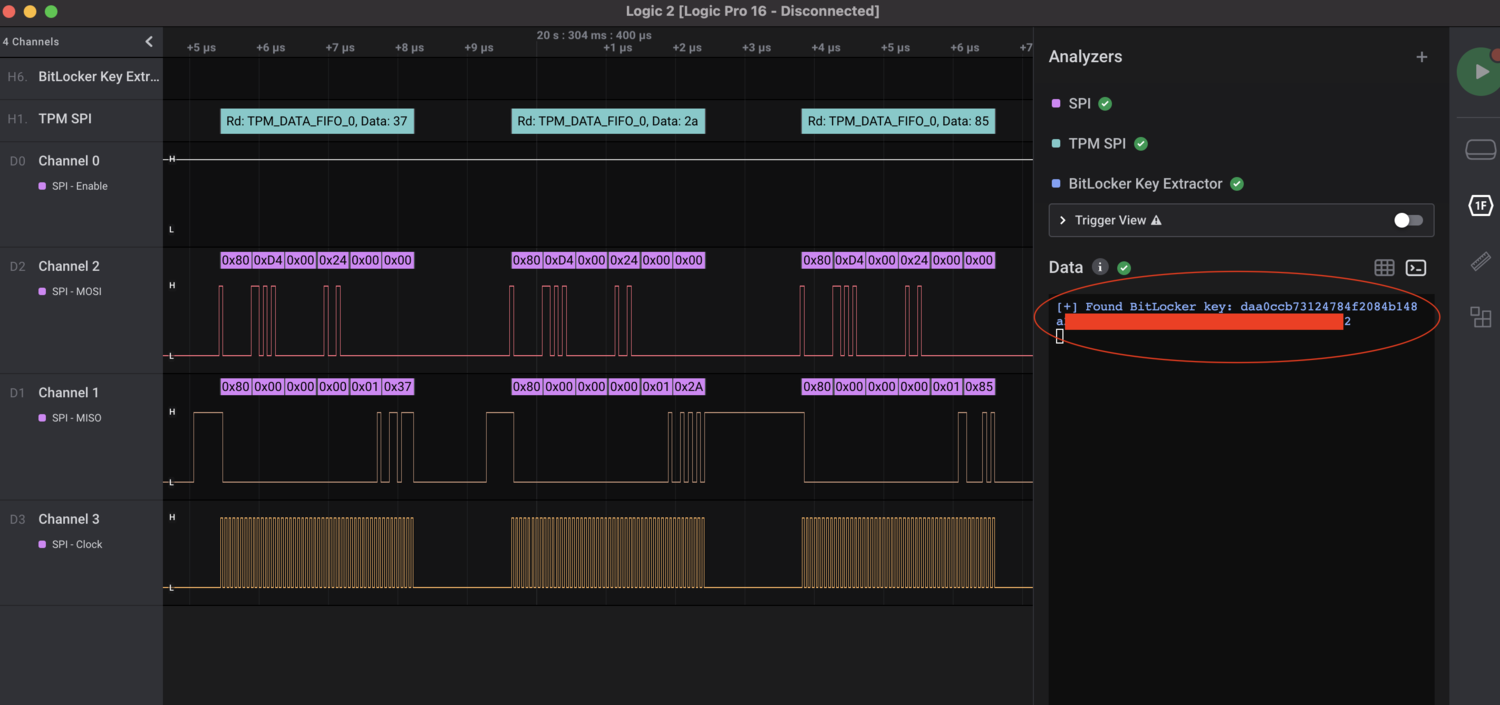
\includegraphics[width=0.8\linewidth]{logic-capture}
			\caption{Saleae Logic Pro \cite{.15122021}}
		\end{figure}
	\end{frame}
	
	\begin{frame}{Speichermedium entschlüsseln}
				\begin{figure}[h!]
			\centering
			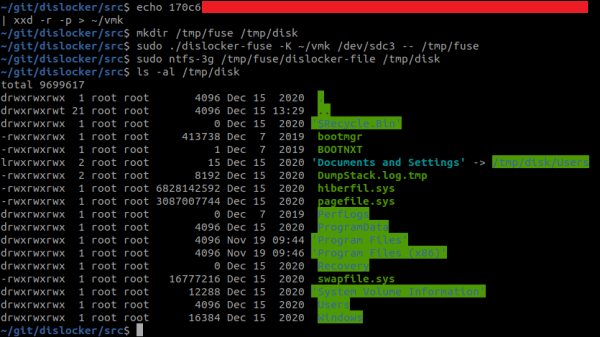
\includegraphics[width=0.8\linewidth]{mount}
			\caption{Dislocker \cite{.16122020b}}
		\end{figure}
		
	\end{frame}

	
	\section{Fazit}
	
	\begin{frame}{Evaluation}
		\begin{itemize}[<+- | alert@+>]
			\item Zeit
			\item Ressourcen
			\item Kosten
			\item Schwierigkeit
		\end{itemize}		
	\end{frame}
	
	\begin{frame}{Prävention}
		\begin{itemize}[<+- | alert@+>]
			\item Zusätzliche Benutzerverifikation
			\item Einschränkung physikalischer Zugriff
		\end{itemize}		
	\end{frame}
	
	\begin{frame}[standout]
		Fragen?
	\end{frame}

	\begin{frame}[allowframebreaks]{Literatur}
		  \bibliography{TPM}
  			\bibliographystyle{abbrv}
	\end{frame}

\end{document}
